\documentclass[a4paper,11pt,final]{article}
% Pour une impression recto verso, utilisez plutôt ce documentclass :
%\documentclass[a4paper,11pt,twoside,final]{article}

\usepackage[english,francais]{babel}
\usepackage[utf8]{inputenc}
\usepackage[T1]{fontenc}
\usepackage[pdftex]{graphicx}
\usepackage{setspace}
\usepackage{hyperref}
\usepackage[french]{varioref}

\newcommand{\reporttitle}{Exemple de rapport}     % Titre
\newcommand{\reportauthor}{Bruno \textsc{Voisin}} % Auteur
\newcommand{\reportsubject}{Stage de fin d'étude} % Sujet
\newcommand{\HRule}{\rule{\linewidth}{0.5mm}}
\setlength{\parskip}{1ex} % Espace entre les paragraphes

\hypersetup{
    pdftitle={\reporttitle},%
    pdfauthor={\reportauthor},%
    pdfsubject={\reportsubject},%
    pdfkeywords={rapport} {vos} {mots} {clés}
}

\begin{document}
  % Inspiré de http://en.wikibooks.org/wiki/LaTeX/Title_Creation

\begin{titlepage}

\begin{center}

\begin{minipage}[t]{0.48\textwidth}
  \begin{flushleft}
    
\includegraphics [width=30mm]{images/logo-univ.jpg} \\[0.5cm]
    \begin{spacing}{1.5}
      \textsc{\LARGE Université de ...}
    \end{spacing}
  \end{flushleft}
\end{minipage}
\begin{minipage}[t]{0.48\textwidth}
  \begin{flushright}
    
\includegraphics [width=30mm]{images/logo-societe.jpg} \\[0.5cm]
    \textsc{\LARGE Entreprise}
  \end{flushright}
\end{minipage} \\[1.5cm]

\textsc{\Large \reportsubject}\\[0.5cm]
\HRule \\[0.4cm]
{\huge \bfseries \reporttitle}\\[0.4cm]
\HRule \\[1.5cm]

\begin{minipage}[t]{0.3\textwidth}
  \begin{flushleft} \large
    \emph{Auteur :}\\
    \reportauthor
  \end{flushleft}
\end{minipage}
\begin{minipage}[t]{0.6\textwidth}
  \begin{flushright} \large
    \emph{Responsables :} \\
    M.~Jean \textsc{Machin} \\
    M.~Pierre \textsc{Bidon}
  \end{flushright}
\end{minipage}

\vfill

{\large 17 novembre 2011}

\end{center}

\end{titlepage}

  \cleardoublepage % Dans le cas du recto verso, ajoute une page blanche si besoin
  \tableofcontents % Table des matières
  \sloppy          % Justification moins stricte : des mots ne dépasseront pas des paragraphes
  \cleardoublepage
  \chapter*{Remerciements}
\addcontentsline{toc}{chapter}{Remerciements}

\paragraph{}
Tout d'abord, je tiens à remercier Stéphanie \textsc{Amar}, ma maître d'apprentissage, pour m'avoir accepté dans son équipe.
Je me dois également de remercier Loïc \textsc{Laine}, technico-commercial, et Jacques \textsc{Semoun}, logisticien intégrateur, pour m'avoir aidé lors de mes difficultés. 
Un grand merci également aux techniciens de Spie qui m'ont énormément appris, tant sur l'aspect professionnel que sur l'aspect social d'une entreprise.
\paragraph{}
Je voudrais également exprimer ma gratitude à la grande famille des \foreignlanguage{english}{Cast Members\footnote{Employés de Disneyland}} pour m'avoir invité dans le monde merveilleux de Walt \textsc{Disney}.
\paragraph{}
Un dernier remerciement à M.~Chan \textsc{Leduc}, à M.~Philippe \textsc{Bonnot} ainsi qu'a tous mes professeurs sans qui je n'aurais pas su répondre aux attentes de l'entreprise.
\paragraph{}
\newacronym{cfa}{CFA}{Centre de Formation des Apprentis}
% \newglossaryentry{CFA}{name={CFA},description={Centre de Formation des Apprentis}}
Je n'oublie pas non plus Mme.~Jocelyne \textsc{Capmal}, ainsi que tous les membres du \gls{cfa}\footnote{Centre de Formation des Apprentis} AFIA, qui nous ont aidé, mes camarades et moi, à trouver une entreprise.

% \chapter*{Thanks}
% \addcontentsline{toc}{chapter}{Thanks}

% \paragraph{}
% First, I want to thanks Stéphanie \textsc{Amar}, my internship master, for giving me the chance to be in his team.
% I have to thanks Loïc \textsc{Laine}, a technico-commercial, and Jacques \textsc{Semoun}, the logistics integrator, for help me when I was in troubles.
% Also a big thanks to the entire team of techniciens of Spie who learn me a lots of things, in the professional aspect as well as in the social aspect of an enterprise.
% \paragraph{}
% \newglossaryentry{Cast Members}{name={Cast Members},description={Employés de Disneyland}}
% I want to tell my gratitude to the great family of the \gls{Cast Members} for inviting me in the wonderfull world of Walt \textsc{Disney}.
% \paragraph{}
% A last thanks to M.~Chan \textsc{Leduc}, and M.~Philippe \textsc{Bonnot}, and to all my teachers without who I couldn't answer to the expectations of the company.
% \paragraph{}
% I don't forget Mme.~Jocelyne \textsc{Capmal}, and all the members of the \gls{CFA} AFIA which help us, my comrade and me, to find out a company.

  \cleardoublepage
  \section*{Introduction}
\addcontentsline{toc}{section}{Introduction}

Cet article est d�stin� � favoriser la prise en main de gEDA, suite libre de Conception �lectronique Assist� par Ordinateur.
Ce n'est en aucun cas une documentation suffisante, il a pour but de compl�ter les articles r�dig�s par les concepteurs.

Nous verrons �galement de quel mani�re programmer les PIC (microcontr�leurs de chez Microchip) sous Linux en C. 

Finalement nous �tudierons les cartes �lectroniques permettant la mesure d'une temp�rature avec les sondes Pt100.

 

  \cleardoublepage
  \section{La première section}


\subsection{Une sous section}

On peut mettre des mots en \emph{italique}, 
en \textsc{petites Majuscules} ou 
en \texttt{largeur fixe (machine à écrire)}.

Voici un deuxième paragraphe avec une formule mathématique simple : $e = mc^2$.

Un troisième avec des \og guillemet français \fg{}.

\subsubsection{Écrire en anglais}

\foreignlanguage{english}{Do you speak French? Does anybody here speak french?}


\subsection{Lites}

\begin{itemize}
\item Liste classique ;
\item un élément ;
\item et un autre élément.
\end{itemize}
\vspace{\parskip} % espace entre paragraphes

\begin{enumerate}
\item Une liste numéroté
\item deux
\item trois
\end{enumerate}
\vspace{\parskip}

\begin{description}
\item[Description] C'est bien pour des définitions.
\item[Deux] Ou pour faire un liste spéciale.
\end{description}
\vspace{\parskip}


\subsection{Références}

Voici une référence à l'image de la figure \ref{bloghiko} page \pageref{bloghiko} et une autre vers la partie \ref{p2} page \pageref{p2}.

On peut citer un livre\,\up{\cite{lpp}} et on précise les détails à la fin du rapport dans la partie références.


\subsection{Note de bas de page}

Voici une note\,\footnote{Texte de bas de page} de bas de page.
Une deuxième\,\footnotemark{} déclarée différemment.
La même note\,\footnotemark[\value{footnote}].

\footnotetext{Il a deux références vers cette note}


\subsection{Figure}

\begin{figure}[!ht]
    \center
    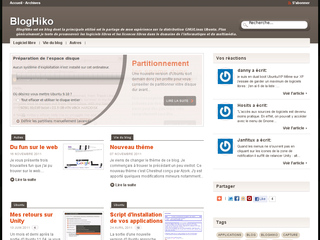
\includegraphics[]{./images/bloghiko.jpg}
    \caption{BlogHiko | taille original}
    \label{bloghiko}
\end{figure}

\begin{figure}[!ht]
    \center
    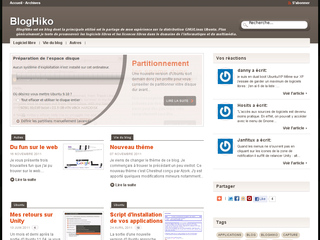
\includegraphics[width=0.5\textwidth]{./images/bloghiko.jpg}
    \caption{BlogHiko | 50\% de la largeur de la page}
\end{figure}


  \cleardoublepage
  \section{Citation Wikipédia}
\label{p2}


LaTeX est un langage et un système de composition de documents créé par Leslie Lamport en 198312. Plus exactement, il s'agit d'une collection de macro-commandes destinées à faciliter l'utilisation du \og processeur de texte \fg{} TeX de Donald Knuth. Depuis 1993, il est maintenu par le LaTeX3 Project team. La première version utilisée largement, appelée LaTeX2.09, est sortie en 1984. Une révision majeure, appelée LaTeX2 epsilon est sortie en 1991.

Le nom est l'abréviation de Lamport TeX. On écrit souvent \LaTeX, le logiciel permettant les mises en forme correspondant au logo.

Du fait de sa relative simplicité, il est devenu la méthode privilégiée d'écriture de documents scientifiques employant TeX. Il est particulièrement utilisé dans les domaines techniques et scientifiques pour la production de documents de taille moyenne ou importante (thèse ou livre, par exemple). Néanmoins, il peut aussi être employé pour générer des documents de types variés (par exemple, des lettres, ou des transparents).


  \cleardoublepage
  \section*{Conclusion}
\addcontentsline{toc}{section}{Conclusion}

Pour conclure, avec \LaTeX{} on obtient un rendu impeccable mais il faut s'investir pour le prendre en main.

  \cleardoublepage
  \chapter*{Références}
\addcontentsline{toc}{chapter}{Références}

\end{document}
